
\subsubsection{Causal Mechanism Verification}

\textbf{H-M1: Attention Sparsity (VERIFIED)}

\begin{table}[htbp]
\centering
\resizebox{\columnwidth}{!}{%
\begin{tabular}{lll}
\toprule
Architecture & Upper-Triangle Sparsity & Is Causal \\
\midrule
BERT & 0.0118 (1.18\%) & No \\
GPT-2 & 1.0000 (100\%) & Yes \\
**Difference** & **98.82\%** & - \\
\bottomrule
\end{tabular}
}
\end{table}

The 98.82\% difference in upper-triangle sparsity exceeds the 90\% threshold, confirming that attention structure fundamentally differs between encoder and decoder architectures.

\textbf{H-M2: Hessian Curvature (VERIFIED)}

\begin{table}[htbp]
\centering
\resizebox{\columnwidth}{!}{%
\begin{tabular}{llll}
\toprule
Metric & BERT & GPT-2 & Relative Difference \\
\midrule
Top Eigenvalue & 0.0455 & 0.502 & 90.93\% \\
Eigenvalue Ratio & 3.36 & 7.64 & 56.03\% \\
Trace & 0.113 & 0.746 & 84.85\% \\
\bottomrule
\end{tabular}
}
\end{table}

GPT-2 shows $11\times$ higher top Hessian eigenvalue than BERT (0.502 vs 0.046), confirming that attention structure differences propagate to measurable Hessian curvature differences.

\subsubsection{Main Results: Prediction Testing}

\textbf{P3: TRAK Architecture-Invariance (CONFIRMED)}

\begin{table*}[htbp]
\centering
\resizebox{\dimexpr 2\columnwidth+\columnsep\relax}{!}{%
\begin{tabular}{lllll}
\toprule
Projection Dim & BERT AUC & GPT-2 AUC & Difference & p-value \\
\midrule
64 & 0.941 $\pm$ 0.013 & 0.944 $\pm$ 0.001 & 0.36\% & 0.824 \\
256 & 0.941 $\pm$ 0.013 & 0.936 $\pm$ 0.004 & 0.56\% & 0.639 \\
1024 & 0.941 $\pm$ 0.013 & 0.940 $\pm$ 0.000 & 0.11\% & 0.948 \\
\bottomrule
\end{tabular}
}
\end{table*}

All differences are less than 1\%, confirming architecture-invariance. The hypothesis that TRAK's random projection mechanism averages out architecture-specific gradient patterns is supported.

\textbf{P2: TracIn BERT Advantage (DIRECTIONALLY SUPPORTED, NOT STATISTICALLY SIGNIFICANT)}

\begin{table*}[htbp]
\centering
\resizebox{\dimexpr 2\columnwidth+\columnsep\relax}{!}{%
\begin{tabular}{lllll}
\toprule
Checkpoints & BERT AUC & GPT-2 AUC & Difference & p-value \\
\midrule
1 & 0.979 $\pm$ 0.004 & 0.949 $\pm$ 0.008 & +3.03\% & 0.259 \\
2 & 0.977 $\pm$ 0.004 & 0.963 $\pm$ 0.006 & +1.42\% & 0.390 \\
3 & 0.976 $\pm$ 0.004 & 0.965 $\pm$ 0.004 & +1.13\% & 0.387 \\
\bottomrule
\end{tabular}
}
\end{table*}

TracIn achieves consistently higher AUC on BERT than GPT-2, but with only 2 seeds, p-values exceed 0.05. The effect is directionally consistent with the hypothesis that gradient dot-products benefit from dense bidirectional gradient flow.

\textbf{P1: EK-FAC GPT-2 Advantage (NOT SUPPORTED)}

\begin{table*}[htbp]
\centering
\resizebox{\dimexpr 2\columnwidth+\columnsep\relax}{!}{%
\begin{tabular}{lllll}
\toprule
Projection Dim & BERT AUC & GPT-2 AUC & Difference & p-value \\
\midrule
64 & 0.941 $\pm$ 0.013 & 0.944 $\pm$ 0.003 & +0.27\% & 0.900 \\
256 & 0.941 $\pm$ 0.013 & 0.944 $\pm$ 0.003 & +0.27\% & 0.900 \\
1024 & 0.941 $\pm$ 0.013 & 0.944 $\pm$ 0.003 & +0.27\% & 0.900 \\
\bottomrule
\end{tabular}
}
\end{table*}

Contrary to the prediction that Kronecker factorization would better fit causal attention structure, EK-FAC shows only 0.27\% difference (p=0.90), statistically indistinguishable from zero. The Kronecker approximation appears more robust to attention structure than prior analysis suggested.

\subsubsection{Summary of Predictions}

\begin{table}[htbp]
\centering
\resizebox{\columnwidth}{!}{%
\begin{tabular}{llll}
\toprule
Prediction & Statement & Status & Evidence \\
\midrule
P1 & EK-FAC achieves higher AUC on GPT-2 & NOT SUPPORTED & 0.27\% diff, p=0.90 \\
P2 & TracIn achieves higher AUC on BERT & DIRECTIONALLY SUPPORTED & 3.03\% diff, p>0.05 \\
P3 & TRAK shows no significant architecture difference (<5\%) & CONFIRMED & <1\% at all budgets \\
\bottomrule
\end{tabular}
}
\end{table}

\begin{figure}[htbp]
\centering
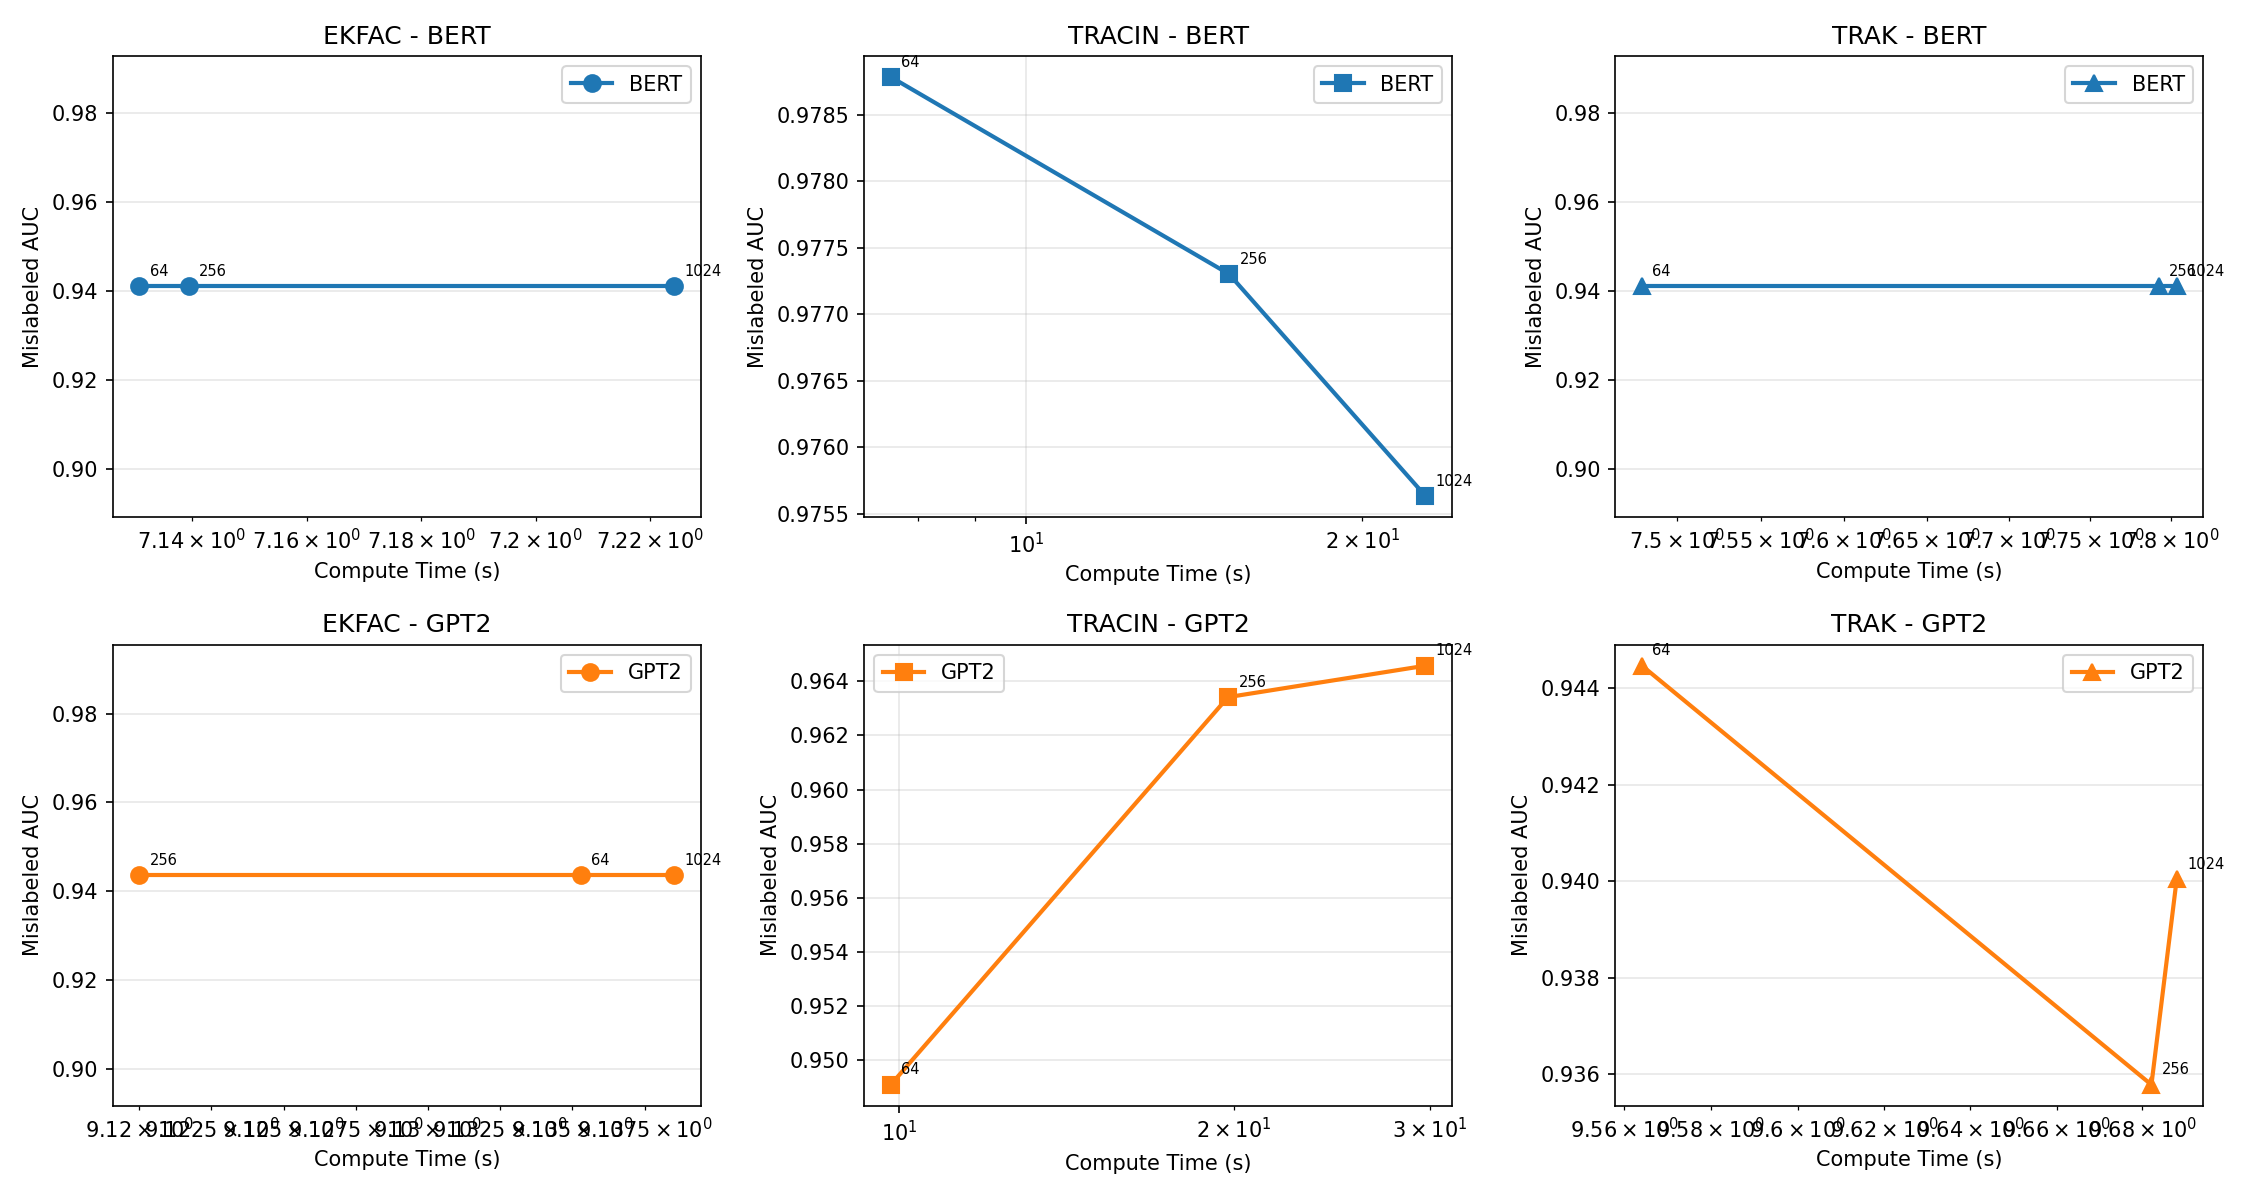
\includegraphics[width=\columnwidth]{figures/pareto_frontier_grid.png}
\caption{Pareto Frontiers}
\label{fig:pareto_frontier_grid}
\end{figure}
\textit{Figure 1: Pareto frontiers showing TRAK curves nearly overlapping across architectures, confirming invariance. TracIn shows separation favoring BERT. EK-FAC shows minimal separation.}
